
\section{Selective Harmonic Elimination as dynamical system}

%


Inspirados en la naturaleza continua de la variable de optimización $f(\tau)$ proponemos en este documento la formulación desde el control óptimo. Es decir en lugar buscar los ángulos de conmutación, buscaremos la función $f(\tau) \in \{ g(\tau)  \in L^\infty([0,\pi])\ /\ |g(\tau)| < 1\} $ que tenga los coeficientes de Fourier deseados. 
%
Utilizaremos el  teorema fundamental del cálculo diferencial para re-escribir la expresión de los coeficientes de Fourier (\ref{an}) y (\ref{bn}) como la evolución de un sistema dinámico. Es decir:

\begin{gather}
    \alpha_i(\tau) = \frac{2}{\pi}\int_0^\tau f(\tau) \cos(i\tau)d\tau 
    \Rightarrow
    \begin{cases} \label{ode}
        \dot{\alpha_i}(\tau) & = \frac{2}{\pi}f(\tau)\cos(i\tau) \\  
        \alpha_i(0) & = 0       
    \end{cases}
\end{gather}

\begin{gather}
    \beta_j(\tau) = \frac{2}{\pi}\int_0^\tau f(\tau) \sin(j\tau)d\tau 
    \Rightarrow
    \begin{cases} \label{ode}
        \dot{\beta}_j(\tau) & = \frac{2}{\pi}f(\tau)\sin(j\tau) \\  
        \beta_j(0) & = 0       
    \end{cases}
\end{gather}

La evolución de los sistemas dinámicos $\alpha_i(\tau)$ y $\beta_j(\tau)$ desde el tiempo $\tau=0$ hasta $\tau=\pi$ nos da lugar a los coeficientes $a_i$ y $b_j$. 
De esta manera, el problema general de SHE (\ref{SHEp}) puede formularse como un problema de control de un sistema dinámico donde $\alpha_i(\tau) \ | \ \forall i \in \mathcal{E}_a  $ y $ \beta_j(\tau) \ \forall j \in \mathcal{E}_b$ son los estados del sistema y donde $f(\tau)$ es la variable de control, y cuyo objetivo será llevar los estados desde el origen de coordenadas hasta los vectores objetivos $\bm{a}_T$ y $\bm{b}_T$ en tiempo $\tau = \pi$ (véase figura (\ref{syscon})).

\subsection{Notación}

Con el fin de obtener una expresión compacta del problema que nos simplifique el entendimiento del mismo introduciremos la siguiente notación 


\begin{gather}
    \bm{x}(t) = [\bm{\alpha}(t) \ , \ \bm{\beta}(t)]^T  
\end{gather}
\begin{gather}
    \bm{x}_T = [\bm{a}_T,\bm{b}_T]^T  
\end{gather}
\begin{gather}
    \bm{\mathcal{D}}(t) = \frac{2}{\pi} \begin{bmatrix}
        \cos(\tau) ,
        \cos(3\tau) ,
        ... ,
        \sin(\tau) ,
        \sin(3\tau) ,
        ... 
    \end{bmatrix}^T
\end{gather}

De manera que para un par de conjuntos $\mathcal{E}_a$ y $\mathcal{E}_b$ tenemos el siguiente sistema dinámico asociado:

\begin{gather}
    \begin{cases}
        \dot{\bm{x}}(t) = \bm{\mathcal{D}}(t)f(t) & \tau \in [0,\pi]\\
        \bm{x}(0) = \bm{0}
    \end{cases}
\end{gather}

\begin{figure}
    \centering
    \begin{subfigure}[b]{0.475\textwidth}
        \centering
        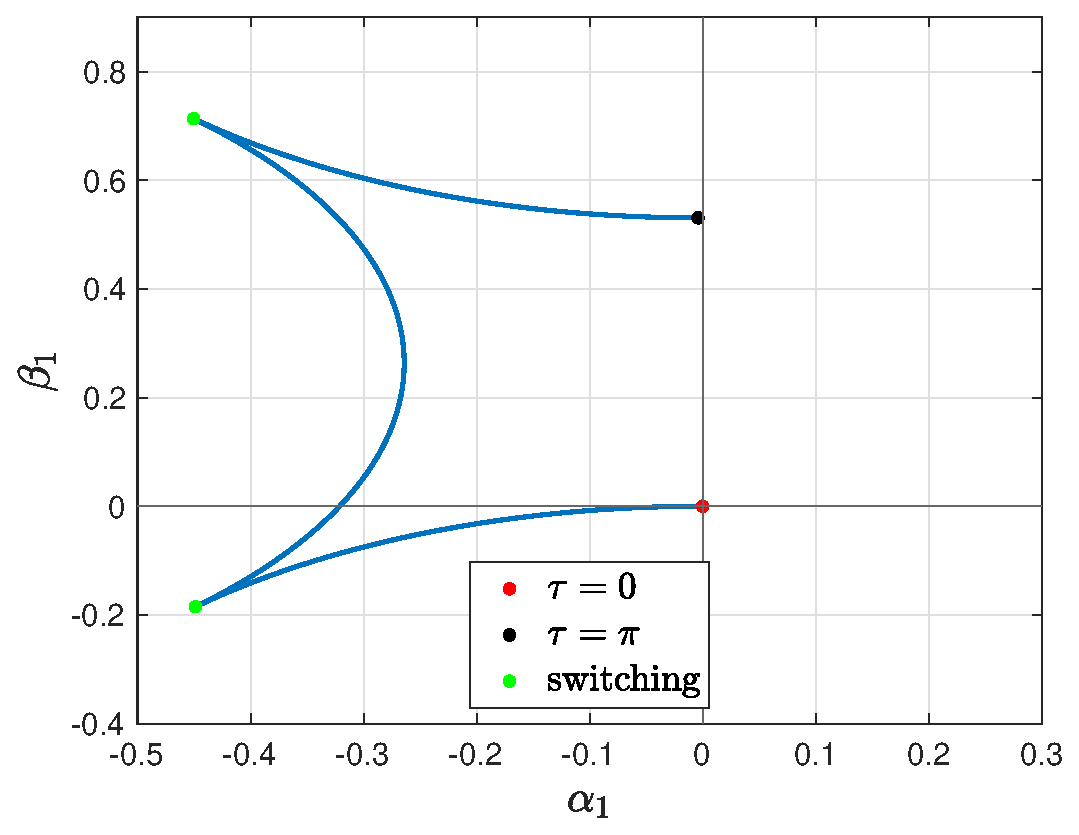
\includegraphics[width=\textwidth]{img/sys.eps}
        \caption{Dynamical System}
        \label{fig:sys}
    \end{subfigure}
    \hfill
    \begin{subfigure}[b]{0.475\textwidth}
        \centering
        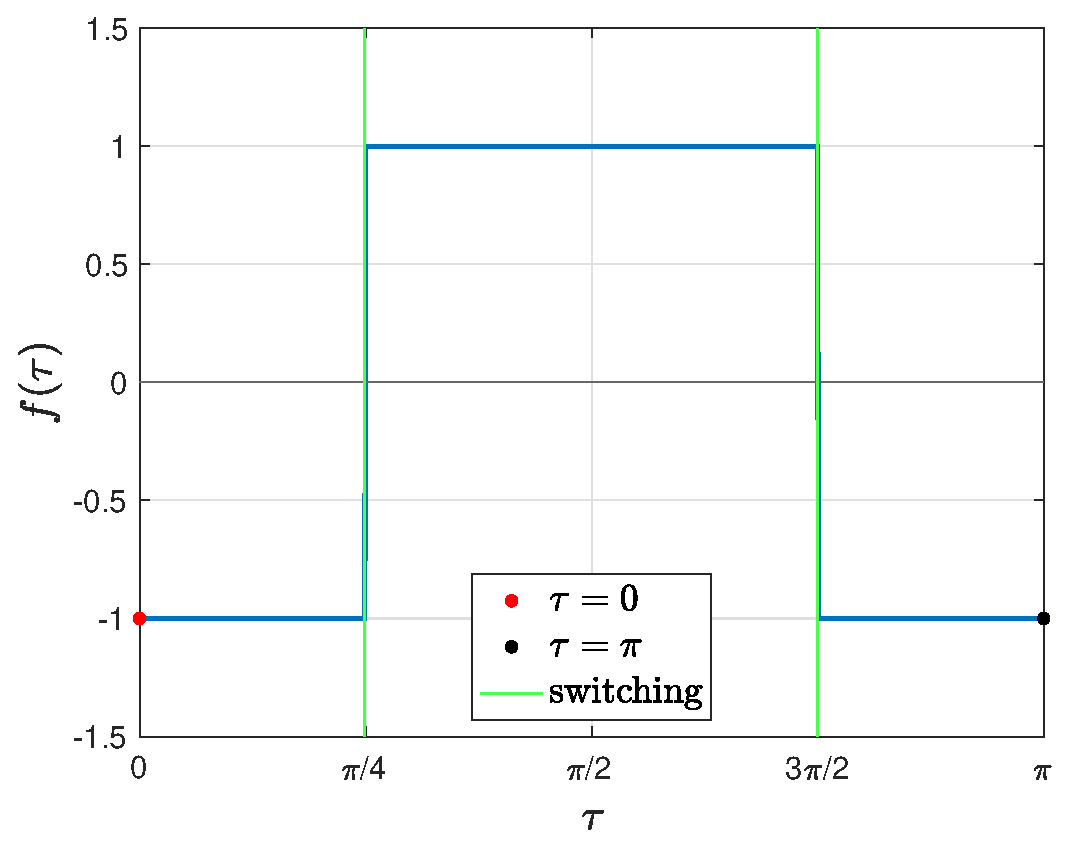
\includegraphics[width=\textwidth]{img/con.eps}
        \caption{Control}
        \label{fig:con}
    \end{subfigure}
    \caption{Mostramos el problema SHE como un sistema dinámico cuando consideramos los coeficientes de Fourier $a_1$ y $b_1$. En la figura (a) podemos ver la evolución del sistema dinámico asociado a los coeficientes de Fourier $a_1$ y $b_1$. Por otro lado, en la figura (b) podemos ver el control $f(\tau)$ que genera la trayectoria mostrada en (a).}
    \label{syscon}
\end{figure}